\chapter{Enfoque Propuesto}
\label{chap:proposed}

Los codificadores de video tienen como tarea fundamental mejorar la eficiencia de codificaci\'on, es decir, minimizar la cantidad de bits que representan un video, maximizando el nivel calidad, teniendo en cuenta las caracter\'isticas de complejidad computacional y un retraso entre el proceso de codificaci\'on (transformar la se\~nal de video en un flujo de bits) y el proceso de decodificaci\'on (reconstruir la se\~nal en base al flujo de bits con cierta p\'erdida de informaci\'on). Usando  t\'ecnicas de CS, se puede representar la informaci\'on que compone el video (un frame, un fragamento del frame, el residual entre la imagen original y su predicci\'on) mediante un diccionario y un vector disperso. El vector disperso es construido resolviendo un problema de minimizaci\'on de la norma $\ell_p$ y el diccionario es construido seleccionando muestras aleatorias de la se\~nal o con un algoritmo de entrenamiento.

En este proyecto se trabaja el problema de la selecci\'on del diccionario para hallar la representaci\'on dispersa de una se\~nal dentro de un proceso de CS para mejorar la eficiencia de codificaci\'on de video. Para resolver este problema, se busca construir un modelo que integre en la selecci\'on del diccionario, los m\'etodos de codificaci\'on perceptual, los cuales tienen en cuentan caracter\'isticas del HVS para seleccionar regiones del video con una mayor importancia para el usuario final. Con estas regiones se pretende inicializar el diccionario para hallar la representaci\'on dispersa de la se\~nal y tambi\'en definir en que punto del video se debe actualizar nuevamente el diccionario. En la propuesta se debe evaluar la rapidez con que converge la aproximaci\'on de la se\~nal (cuantas iteraciones se deben realizar para hallar la representaci\'on dispersa) y el error entre la se\~nal reconstruida y la original. En la figura \ref{fig:proposed_sparse} se presenta un esquema con las ideas b\'asicas del enfoque propuesto.

\begin{figure}[!ht]
\centering
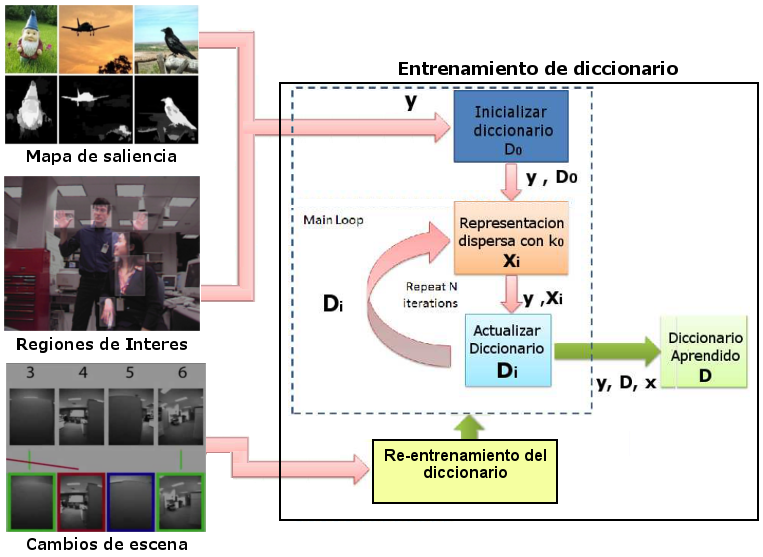
\includegraphics[width=0.7\textwidth]{images/propuesta.png}
\caption{Esquema del modelo base del enfoque propuesto }
\label{fig:proposed_sparse}
\end{figure}

El modelo propuesto debe ser implementado e integrado a un est\'andar de codificaci\'on de video. En el componente de codificaci\'on se debe hallar la representaci\'on dispersa del video y en en el componente de decodificaci\'on se debe reconstruir el video respecto al diccionario y los vectores dispersos. Respecto a los est\'andares de codificaci\'on, se debe seleccionar entre el HEVC o el vp9, ya que son los m\'as representativos en la actualidad. Dada estas condiciones, el diccionario y los vectores dispersos deben ser transmitidos al decodificador para la reconstrucci\'on, por lo tanto se debe usar una estrategia para la transmisi\'on, bien sea insert\'andolos dentro del flujo de bits generado por el codificador o transmitirlos de forma independiente. Tambi\'en se debe revisar la opci\'on de codificar el diccionario para minimizar el tama\~no del diccionario y los vectores dispersos. 

Para evaluar el impacto del modelo propuesto en el proceso de codificaci\'on, se deben tener en cuenta la tasa de bits del video, algunas m\'etricas de calidad objetiva, como la Relación Señal a Ruido de Pico (PSNR) o la similaridad estructural (SSIM), y algunas m\'etricas de calidad subjetiva como el puntaje medio de opini\'on (MOS). Tambi\'en se debe evaluar el rendimiento computacional de la propuesta en t\'erminos del tiempo que tarda en realiza el proceso de codificaci\'on y decodificaci\'on. Todas estas caracter\'isticas deben ser comparadas con los resultados de un modelo de referencia del est\'andar de codificaci\'on el cual no tenga modificaciones, y de esta forma revisar el impacto del modelo propuesto. 

Aunque algunas propuestas han usado la percepci\'on visual en modelos de CS para video, estas no han integrado directamente la codificaci\'on perceptual al proceso de selecci\'on del diccionario. Con la implementaci\'on e integraci\'on del modelo propuesto se espera que el diccionario permita hallar la representaci\'on dispersa de la se\~nal m\'as r\'apido en comparaci\'on a otros m\'etodos de selecci\'on y entrenamiento de diccionarios. Tambi\'en se espera reducir la tasa de bits, manteniendo los niveles de calidad del video, con un impacto m\'inimo en el tiempo computacional del proceso de codificaci\'on.

